\documentclass{standalone}
\usepackage{tikz}
\usetikzlibrary{patterns, positioning}

\begin{document}
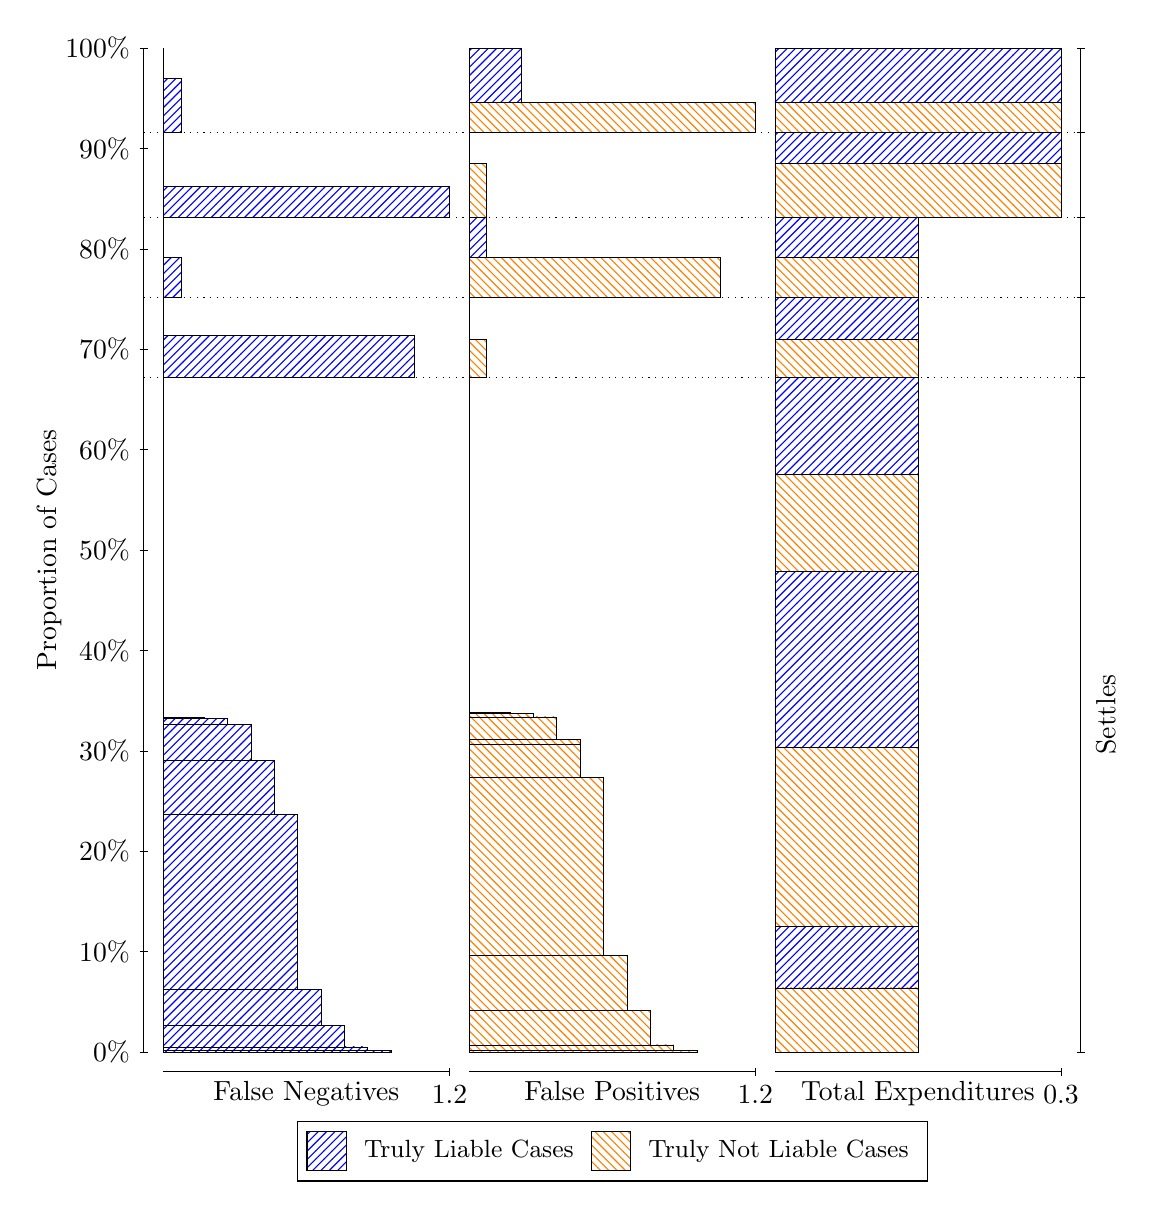
\begin{tikzpicture}
\draw[black, very thin] (1.5,1.75) -- (1.5,14.5);
\node[rotate=90, anchor=center] at (0.3, 8.125) {Proportion of Cases};
\draw[black, very thin] (1.45,1.75) -- (1.55,1.75);
\node[anchor=east] at (1.45, 1.75) {0\%};
\draw[black, very thin] (1.45,3.025) -- (1.55,3.025);
\node[anchor=east] at (1.45, 3.025) {10\%};
\draw[black, very thin] (1.45,4.3) -- (1.55,4.3);
\node[anchor=east] at (1.45, 4.3) {20\%};
\draw[black, very thin] (1.45,5.575) -- (1.55,5.575);
\node[anchor=east] at (1.45, 5.575) {30\%};
\draw[black, very thin] (1.45,6.85) -- (1.55,6.85);
\node[anchor=east] at (1.45, 6.85) {40\%};
\draw[black, very thin] (1.45,8.125) -- (1.55,8.125);
\node[anchor=east] at (1.45, 8.125) {50\%};
\draw[black, very thin] (1.45,9.4) -- (1.55,9.4);
\node[anchor=east] at (1.45, 9.4) {60\%};
\draw[black, very thin] (1.45,10.675) -- (1.55,10.675);
\node[anchor=east] at (1.45, 10.675) {70\%};
\draw[black, very thin] (1.45,11.95) -- (1.55,11.95);
\node[anchor=east] at (1.45, 11.95) {80\%};
\draw[black, very thin] (1.45,13.225) -- (1.55,13.225);
\node[anchor=east] at (1.45, 13.225) {90\%};
\draw[black, very thin] (1.45,14.5) -- (1.55,14.5);
\node[anchor=east] at (1.45, 14.5) {100\%};

\draw[black, very thin] (13.4,1.75) -- (13.4,14.5);
\draw[black, very thin] (13.35,1.75) -- (13.45,1.75);
\node[anchor=west] at (13.35, 1.75) {};
\draw[black, very thin] (13.35,10.32) -- (13.45,10.32);
\node[anchor=west] at (13.35, 10.32) {};
\draw[black, very thin] (13.35,11.332) -- (13.45,11.332);
\node[anchor=west] at (13.35, 11.332) {};
\draw[black, very thin] (13.35,12.353) -- (13.45,12.353);
\node[anchor=west] at (13.35, 12.353) {};
\draw[black, very thin] (13.35,13.424) -- (13.45,13.424);
\node[anchor=west] at (13.35, 13.424) {};
\draw[black, very thin] (13.35,14.5) -- (13.45,14.5);
\node[anchor=west] at (13.35, 14.5) {};

\draw[black, very thin, pattern color=blue, pattern=north east lines] (1.75,1.75) rectangle (4.6418,1.7702);
\draw[black, very thin, pattern color=blue, pattern=north east lines] (1.75,1.7702) rectangle (4.3452,1.8135);
\draw[black, very thin, pattern color=blue, pattern=north east lines] (1.75,1.8135) rectangle (4.0486,2.0907);
\draw[black, very thin, pattern color=blue, pattern=north east lines] (1.75,2.0907) rectangle (3.752,2.5498);
\draw[black, very thin, pattern color=blue, pattern=north east lines] (1.75,2.5498) rectangle (3.4554,4.7666);
\draw[black, very thin, pattern color=blue, pattern=north east lines] (1.75,4.7666) rectangle (3.1588,5.456);
\draw[black, very thin, pattern color=blue, pattern=north east lines] (1.75,5.456) rectangle (2.8622,5.9073);
\draw[black, very thin, pattern color=blue, pattern=north east lines] (1.75,5.9073) rectangle (2.5656,5.9853);
\draw[black, very thin, pattern color=blue, pattern=north east lines] (1.75,5.9853) rectangle (2.269,6.0034);
\draw[black, very thin, pattern color=orange, pattern=north west lines] (1.75,6.0034) rectangle (1.75,10.32);
\draw[black, very thin, pattern color=blue, pattern=north east lines] (1.75,10.32) rectangle (4.9384,10.851);
\draw[black, very thin, pattern color=orange, pattern=north west lines] (1.75,10.851) rectangle (1.75,11.332);
\draw[black, very thin, pattern color=blue, pattern=north east lines] (1.75,11.332) rectangle (1.9724,11.843);
\draw[black, very thin, pattern color=orange, pattern=north west lines] (1.75,11.843) rectangle (1.75,12.353);
\draw[black, very thin, pattern color=blue, pattern=north east lines] (1.75,12.353) rectangle (5.3833,12.743);
\draw[black, very thin, pattern color=orange, pattern=north west lines] (1.75,12.743) rectangle (1.75,13.424);
\draw[black, very thin, pattern color=blue, pattern=north east lines] (1.75,13.424) rectangle (1.9724,14.113);
\draw[black, very thin, pattern color=orange, pattern=north west lines] (1.75,14.113) rectangle (1.75,14.5);
\draw[black, very thin, pattern color=orange, pattern=north west lines] (5.6333,1.75) rectangle (8.5252,1.7679);
\draw[black, very thin, pattern color=orange, pattern=north west lines] (5.6333,1.7679) rectangle (8.2286,1.8414);
\draw[black, very thin, pattern color=orange, pattern=north west lines] (5.6333,1.8414) rectangle (7.932,2.2816);
\draw[black, very thin, pattern color=orange, pattern=north west lines] (5.6333,2.2816) rectangle (7.6354,2.9786);
\draw[black, very thin, pattern color=orange, pattern=north west lines] (5.6333,2.9786) rectangle (7.3388,5.2344);
\draw[black, very thin, pattern color=orange, pattern=north west lines] (5.6333,5.2344) rectangle (7.0422,5.6613);
\draw[black, very thin, pattern color=orange, pattern=north west lines] (5.6333,5.6613) rectangle (7.0422,5.7194);
\draw[black, very thin, pattern color=orange, pattern=north west lines] (5.6333,5.7194) rectangle (6.7456,6.0043);
\draw[black, very thin, pattern color=orange, pattern=north west lines] (5.6333,6.0043) rectangle (6.449,6.0473);
\draw[black, very thin, pattern color=orange, pattern=north west lines] (5.6333,6.0473) rectangle (6.1524,6.0661);
\draw[black, very thin, pattern color=blue, pattern=north east lines] (5.6333,6.0661) rectangle (5.6333,10.32);
\draw[black, very thin, pattern color=orange, pattern=north west lines] (5.6333,10.32) rectangle (5.8558,10.8);
\draw[black, very thin, pattern color=blue, pattern=north east lines] (5.6333,10.8) rectangle (5.6333,11.332);
\draw[black, very thin, pattern color=orange, pattern=north west lines] (5.6333,11.332) rectangle (8.8218,11.842);
\draw[black, very thin, pattern color=blue, pattern=north east lines] (5.6333,11.842) rectangle (5.8558,12.353);
\draw[black, very thin, pattern color=orange, pattern=north west lines] (5.6333,12.353) rectangle (5.8558,13.034);
\draw[black, very thin, pattern color=blue, pattern=north east lines] (5.6333,13.034) rectangle (5.6333,13.424);
\draw[black, very thin, pattern color=orange, pattern=north west lines] (5.6333,13.424) rectangle (9.2667,13.811);
\draw[black, very thin, pattern color=blue, pattern=north east lines] (5.6333,13.811) rectangle (6.3007,14.5);
\draw[black, very thin, pattern color=orange, pattern=north west lines] (9.5167,1.75) rectangle (11.333,2.5629);
\draw[black, very thin, pattern color=blue, pattern=north east lines] (9.5167,2.5629) rectangle (11.333,3.3425);
\draw[black, very thin, pattern color=orange, pattern=north west lines] (9.5167,3.3425) rectangle (11.333,5.6171);
\draw[black, very thin, pattern color=blue, pattern=north east lines] (9.5167,5.6171) rectangle (11.333,7.8541);
\draw[black, very thin, pattern color=orange, pattern=north west lines] (9.5167,7.8541) rectangle (11.333,9.0827);
\draw[black, very thin, pattern color=blue, pattern=north east lines] (9.5167,9.0827) rectangle (11.333,10.32);
\draw[black, very thin, pattern color=orange, pattern=north west lines] (9.5167,10.32) rectangle (11.333,10.8);
\draw[black, very thin, pattern color=blue, pattern=north east lines] (9.5167,10.8) rectangle (11.333,11.332);
\draw[black, very thin, pattern color=orange, pattern=north west lines] (9.5167,11.332) rectangle (11.333,11.842);
\draw[black, very thin, pattern color=blue, pattern=north east lines] (9.5167,11.842) rectangle (11.333,12.353);
\draw[black, very thin, pattern color=orange, pattern=north west lines] (9.5167,12.353) rectangle (13.15,13.034);
\draw[black, very thin, pattern color=blue, pattern=north east lines] (9.5167,13.034) rectangle (13.15,13.424);
\draw[black, very thin, pattern color=orange, pattern=north west lines] (9.5167,13.424) rectangle (13.15,13.811);
\draw[black, very thin, pattern color=blue, pattern=north east lines] (9.5167,13.811) rectangle (13.15,14.5);
\draw[black, dotted] (1.5,10.32) -- (13.4,10.32);
\draw[black, dotted] (1.5,11.332) -- (13.4,11.332);
\draw[black, dotted] (1.5,12.353) -- (13.4,12.353);
\draw[black, dotted] (1.5,13.424) -- (13.4,13.424);
\draw[black, very thin] (1.75,1.5) -- (5.3833,1.5);
\node[anchor=north] at (3.5667, 1.5) {False Negatives};
\draw[black, very thin] (5.3833,1.45) -- (5.3833,1.55);
\node[anchor=north] at (5.3833, 1.45) {1.2};

\draw[black, very thin] (5.6333,1.5) -- (9.2667,1.5);
\node[anchor=north] at (7.45, 1.5) {False Positives};
\draw[black, very thin] (9.2667,1.45) -- (9.2667,1.55);
\node[anchor=north] at (9.2667, 1.45) {1.2};

\draw[black, very thin] (9.5167,1.5) -- (13.15,1.5);
\node[anchor=north] at (11.333, 1.5) {Total Expenditures};
\draw[black, very thin] (13.15,1.45) -- (13.15,1.55);
\node[anchor=north] at (13.15, 1.45) {0.3};

\node[black, centered, rotate=90] at (13.72, 6.0348) {Settles};





\draw (7.449999999999999,1.5) node[draw=none] (baseCoordinate) {};
\begin{scope}[align=center]
        \matrix[scale=0.5, draw=black, below=0.5cm of baseCoordinate, nodes={draw}, column sep=0.1cm]{
            \node[rectangle, draw, minimum width=0.5cm, minimum height=0.5cm, pattern=north east lines, pattern color=blue] {}; &
            \node[draw=none, font=\small] (B) {Truly Liable Cases}; &
            \node[rectangle, draw, minimum width=0.5cm, minimum height=0.5cm, pattern=north west lines, pattern color=orange] {}; &
            \node[draw=none, font=\small] (B) {Truly Not Liable Cases}; \\
            };
\end{scope}

\end{tikzpicture}
\end{document}